\documentclass[14pt]{extbook}
\usepackage{multicol, enumerate, enumitem, hyperref, color, soul, setspace, parskip, fancyhdr} %General Packages
\usepackage{amssymb, amsthm, amsmath, bbm, latexsym, units, mathtools} %Math Packages
\everymath{\displaystyle} %All math in Display Style
% Packages with additional options
\usepackage[headsep=0.5cm,headheight=12pt, left=1 in,right= 1 in,top= 1 in,bottom= 1 in]{geometry}
\usepackage[usenames,dvipsnames]{xcolor}
\usepackage{dashrule}  % Package to use the command below to create lines between items
\newcommand{\litem}[1]{\item#1\hspace*{-1cm}\rule{\textwidth}{0.4pt}}
\pagestyle{fancy}
\lhead{Progress Quiz 9}
\chead{}
\rhead{Version A}
\lfoot{8590-6105}
\cfoot{}
\rfoot{Fall 2020}
\begin{document}

\begin{enumerate}
\litem{
Evaluate the limit below, if possible.\[ \lim_{x \rightarrow 8} \frac{\sqrt{6x - 12} - 6}{3x - 24} \]\begin{enumerate}[label=\Alph*.]
\item \( 0.083 \)
\item \( \infty \)
\item \( 0.167 \)
\item \( 0.028 \)
\item \( \text{None of the above} \)

\end{enumerate} }
\litem{
To estimate the one-sided limit of the function below as $x$ approaches 5 from the right, which of the following sets of numbers should you use?\[ \frac{\frac{5}{x} - 1}{x - 5} \]\begin{enumerate}[label=\Alph*.]
\item \( \{ 4.9000, 4.9900, 4.9990, 4.9999 \} \)
\item \( \{ 4.9000, 4.9900, 5.0100, 5.1000 \} \)
\item \( \{ 5.0000, 5.1000, 5.0100, 5.0010 \} \)
\item \( \{ 5.0000, 4.9000, 4.9900, 4.9990 \} \)
\item \( \{ 5.1000, 5.0100, 5.0010, 5.0001 \} \)

\end{enumerate} }
\litem{
Evaluate the one-sided limit of the function $f(x)$ below, if possible.\[ \lim_{x \rightarrow 3^+} \frac{6}{(x-3)^3}+8 \]\begin{enumerate}[label=\Alph*.]
\item \( -\infty \)
\item \( \infty \)
\item \( f(3) \)
\item \( \text{The limit does not exist} \)
\item \( \text{None of the above} \)

\end{enumerate} }
\litem{
Evaluate the one-sided limit of the function $f(x)$ below, if possible.\[ \lim_{x \rightarrow -7^-} \frac{8}{(x-7)^7}+2 \]\begin{enumerate}[label=\Alph*.]
\item \( -\infty \)
\item \( f(-7) \)
\item \( \infty \)
\item \( \text{The limit does not exist} \)
\item \( \text{None of the above} \)

\end{enumerate} }
\litem{
To estimate the one-sided limit of the function below as $x$ approaches 5 from the left, which of the following sets of numbers should you use?\[ \frac{\frac{5}{x} - 1}{x - 5} \]\begin{enumerate}[label=\Alph*.]
\item \( \{ 5.0000, 4.9000, 4.9900, 4.9990 \} \)
\item \( \{ 5.1000, 5.0100, 5.0010, 5.0001 \} \)
\item \( \{ 4.9000, 4.9900, 5.0100, 5.1000 \} \)
\item \( \{ 4.9000, 4.9900, 4.9990, 4.9999 \} \)
\item \( \{ 5.0000, 5.1000, 5.0100, 5.0010 \} \)

\end{enumerate} }
\litem{
For the graph below, evaluate the limit: $ \displaystyle \lim_{x \rightarrow 3} f(x)$.
\begin{center}
    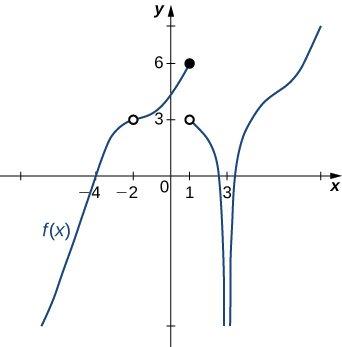
\includegraphics[width=0.5\textwidth]{../Figures/evaluateLimitGraphicallyCopyA.png}
\end{center}
\begin{enumerate}[label=\Alph*.]
\item \( 1 \)
\item \( -\infty \)
\item \( -2 \)
\item \( \text{The limit does not exist} \)
\item \( \text{None of the above} \)

\end{enumerate} }
\litem{
Based on the information below, which of the following statements is always true?\[ As $x$ approaches $\infty$, $f(x)$ approaches $13.506$. \]\begin{enumerate}[label=\Alph*.]
\item \( f(x) \text{ is close to or exactly } 13.506 \text{ when } x \text{ is large enough}. \)
\item \( f(x) \text{ is close to or exactly } \infty \text{ when } x \text{ is large enough}. \)
\item \( f(x) \text{ is undefined when } f(x) \text{ is large enough}. \)
\item \( f(x) \text{ is undefined when } x \text{ is large enough}. \)
\item \( \text{None of the above are always true.} \)

\end{enumerate} }
\litem{
For the graph below, find the value(s) $a$ that makes the statement true: $ \displaystyle \lim_{x \rightarrow a} f(x)$ does not exist.
\begin{center}
    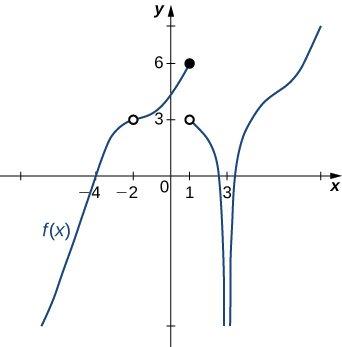
\includegraphics[width=0.5\textwidth]{../Figures/evaluateLimitGraphicallyA.png}
\end{center}
\begin{enumerate}[label=\Alph*.]
\item \( 1 \)
\item \( 3 \)
\item \( -2 \)
\item \( \text{Multiple } a \text{ make the statement true}. \)
\item \( \text{No } a \text{ make the statement true}. \)

\end{enumerate} }
\litem{
Evaluate the limit below, if possible.\[ \lim_{x \rightarrow 9} \frac{\sqrt{3x - 2} - 5}{9x - 81} \]\begin{enumerate}[label=\Alph*.]
\item \( 0.011 \)
\item \( \infty \)
\item \( 0.192 \)
\item \( 0.100 \)
\item \( \text{None of the above} \)

\end{enumerate} }
\litem{
Based on the information below, which of the following statements is always true?\[ As $x$ approaches $1$, $f(x)$ approaches $7.878$. \]\begin{enumerate}[label=\Alph*.]
\item \( f(x) = 7.878 \text{ when } x \text{ is close to } 1 \)
\item \( f(x) \text{ is close to or exactly } 1 \text{ when } x \text{ is close to } 7.878 \)
\item \( f(x) = 1 \text{ when } x \text{ is close to } 7.878 \)
\item \( f(x) \text{ is close to or exactly } 7.878 \text{ when } x \text{ is close to } 1 \)
\item \( \text{None of the above are always true.} \)

\end{enumerate} }
\end{enumerate}

\end{document}